% !TEX root = ../main.tex
\chapter{Optical imaging of non-self-luminous objects}
\begin{figure}[htb]
	\centering
	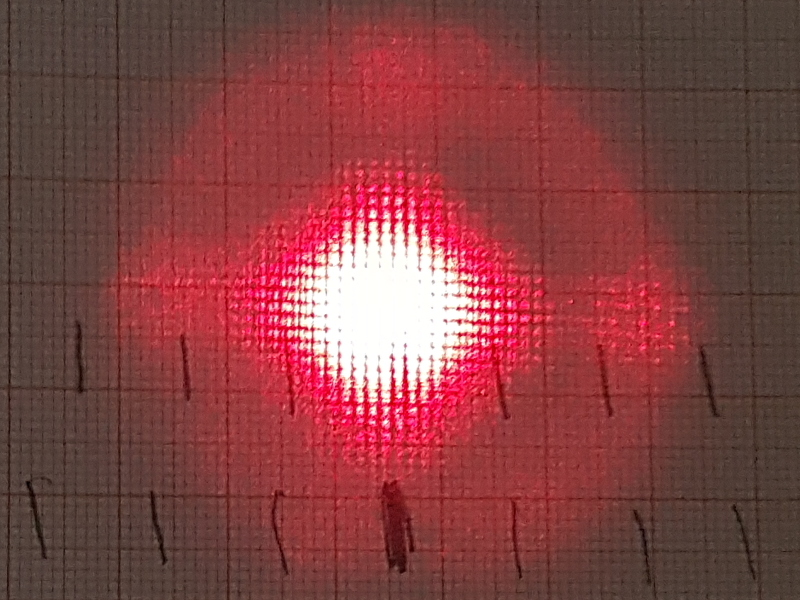
\includegraphics[width=0.6\textwidth]{./img/lattice_struct.jpg}
	\caption[Optical imaging of a lattice]{Optical imaging of a lattice}
	\label{fig:lattice_struct}
\end{figure}

The Abbe theory of imaging states that all orders of diffraction contribute to a correct optical imaging of an object.
This can be demonstrated by illuminating a lattice with a laser and projecting it with a lens onto a distant screen.
Next, a shutter is placed in the focal plane of the lens, which makes it possible to filter out specific diffraction orders.
If the shutter is adjusted so that only the light of $0$-th order can pass it, only a blurred spot is visible on the screen.
However, if higher orders are let through, the lattice structure is clearly visible (see \autoref{fig:lattice_struct}).
It becomes clear that only the higher orders of diffraction carry information of the geometrical object.
